\section{Applications}
This section will consider some of the applications of percolation theory and this idea of critical thresholds --- the idea that there exists a point in a system where the
structure of said system changes massively. Due to the constraints on the length of this essay, I will only go into detail about an application in epidemiology. Howewver, there
are plenty of other applications in such as understanding how forest fires spread \cite{Pak} and how traffic moves around a city. \cite{Li}

\subsection{Epidemiology}
It wouldn't be an essay written in 2020-2021 if I didn't mention epidemiology in one way or another. This part of the essay will focus on and summarise a paper written in 2011 by Eben Kenah and
Joel C. Miller at the University of Washington \cite{Kenah}. The aforementioned paper sets up a Susceptible, Exposed, Infected, Removed (SEIR) model. Every member of the population
is in one of these four states at any given time. If a member of the population is:

\begin{itemize}
  \item susceptible then they're in a position where they could contract the disease
  \item exposed then they have been exposed to the disease and it is currently in a latent period during which the member is infected but not infectious
  \item infected then the member is now infectious with the disease
  \item removed then the member is no longer susceptible to the disease and nor are they infectious.
\end{itemize}

The E and I stages take some time to transition through and in the model are equipped with an $\varepsilon_i$ and a $r_i$ to describe the amount of time it takes to become infectous
after being exposed and the amount of time it takes to recover after becoming infected. Furthermore, we say that the \textit{size} of an epidemic is the total number of people
infected over all time periods and that the \textit{attack rate} of an epidemic is the number of people infected in any given time frame.

The model in this paper is called an Epidemic Percolation Network (EPN) and it relies on representing each individual $i$ in the population as a vertex in a
network. Then for every other $j$ in the population the edge between $i$ and $j$ can be one of the four following things:

\begin{enumerate}
  \item no edge between $i$ and $j$,
  \item a directed edge from $i$ to $j$,
  \item a directed edge from $j$ to $i$,
  \item an undirected edge between $i$ and $j$.
\end{enumerate}

Point 2 means that $i$ will infect $j$ if $i$ is ever infected, point 3 means that $j$ will infect $i$ if $j$ is ever infected, point 4 means that if $i$ is infected then it will infect $j$ or vice
versa and point 1 means that if $i$ is infected it will \textit{not} infect $j$ or vice versa. It's worth noting that these edges are assigned randomly and as a result we have a
random network.

We define the \textit{in-component} of $i$ to be the set of nodes from which $i$ can be reached by choosing the correct path. We also define the \textit{out-component} of $i$ to be the set of nodes that can be reached from $i$
by following a series of edges. In both of these definitions, the undirected edges may be traversed in either direction. The idea for these definitions is that if any node in the
in-component of $i$ is infected then $i$ will eventually be infected and if $i$ is infected then every node in the out-component of $i$ will be infected eventually. As a result of
the randomness of the network, any given individual $i$ does not have a set in- or out-components. We consider the \textit{epidemic threshold} of this SEIR model to correspond to
the emergence of large components in the EPN. We define a \textit{strongly connected component} (SCC) to be a group of nodes wherein each node can be reached by any other node. As a
result of all these nodes being connected, each node in a SCC has the same in- and out-component as every other node in the SCC. As before, the transition in structure occurs when
we go from having a mostly disconnected structure to a mostly connected structure. As such, an EPN below the epidemic threshold gives us many small SCCs, but an EPN
above the epidemic threshold gives us one \textit{giant strongly connected component} (GSCC) and many small SCCs. We lable the in-component of the GSCC as GIN and the
out-component of the GSCC as GOUT. Armed with this extra terminology, we can now see that if all initial infections occur outside the GIN then we have a minor epidemic because the
out-components of all initial infections are small. However, if the initial infection is in the GIN, then the infection necessarily spreads to the GSCC and also to the GOUT so we
have a major epidemic.

This model turns out to be useful for understanding how we should vaccinate the population. This paper tested two pre-vaccination strategies on this network based EPN (i.e.
vaccinating before the start of an outbreak). Strategy 1:
Ranking all nodes in the network by decreasing degree. Strategy 2: Generate a single instance of the EPN and rank all of the nodes in the GSCC by the number of edges connecting
them to other nodes in the GSCC. All other nodes were ranked randomly underneath the nodes in the GSCC. Then in both strategies, the paper chooses some vaccination fraction, $\nu$,
and vaccinates the first $n\nu$ nodes in the list where $n$ is the number of nodes in the population. These strategies were tested on two types of network: Erd\H{o}s-R\'{e}nyi network
with mean degree $5$ and a scale-free network with $\alpha = 2$.

An Erd\H{o}s-R\'{e}nyi network of mean degree $5$ just means that if you sum the degrees of all the nodes and divide that by the number of nodes you should get something close to
5. A scale-free network with $\alpha = 2$ means that the fraction of nodes in the network of degree $k$ is given by $P(k) \sim k^{-\alpha}$.

The paper also adds a methodd for representing the variation in susceptibility and infectiousness between any two given nodes which is represented by the following quantity:

$$p_{ij} = 1 - e^{-100 \times \text{inf}_i \times \text{sus}_j}$$

Where $0 \le \text{inf}_i \le 1$ is the infectiousness of $i$ and $0 \le \text{sus}_j \le 1$ is the susceptibility of $j$. The paper then allowed $\text{inf}_i$ and $\text{sus}_j$
to have different beta distributions. The two cases that were studied for a beta(2, 2) distribution and a beta(0.25, 0.25) distribution. The beta(2, 2) distribution just has one
peak at 0.5 and as a result there isn't much variation in susceptibility and infectiousness. The beta(0.25, 0.25) distribution, however, has peaks at 0 and 1 resulting in nodes
either having very high or very low infectiousness or susceptibility.

\begin{figure}[p]
  \centering
  % 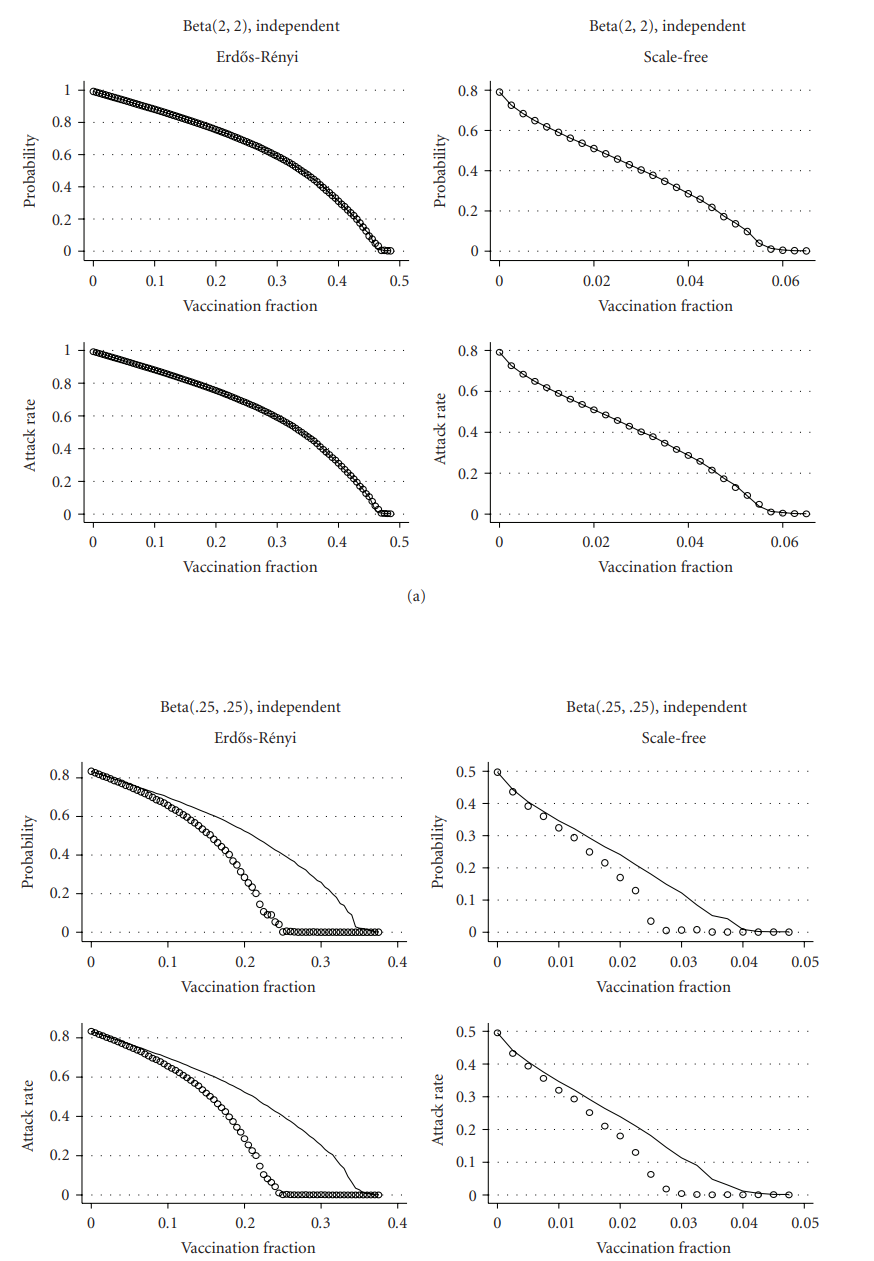
\includegraphics[width=\textwidth]{3/epigraphs}
  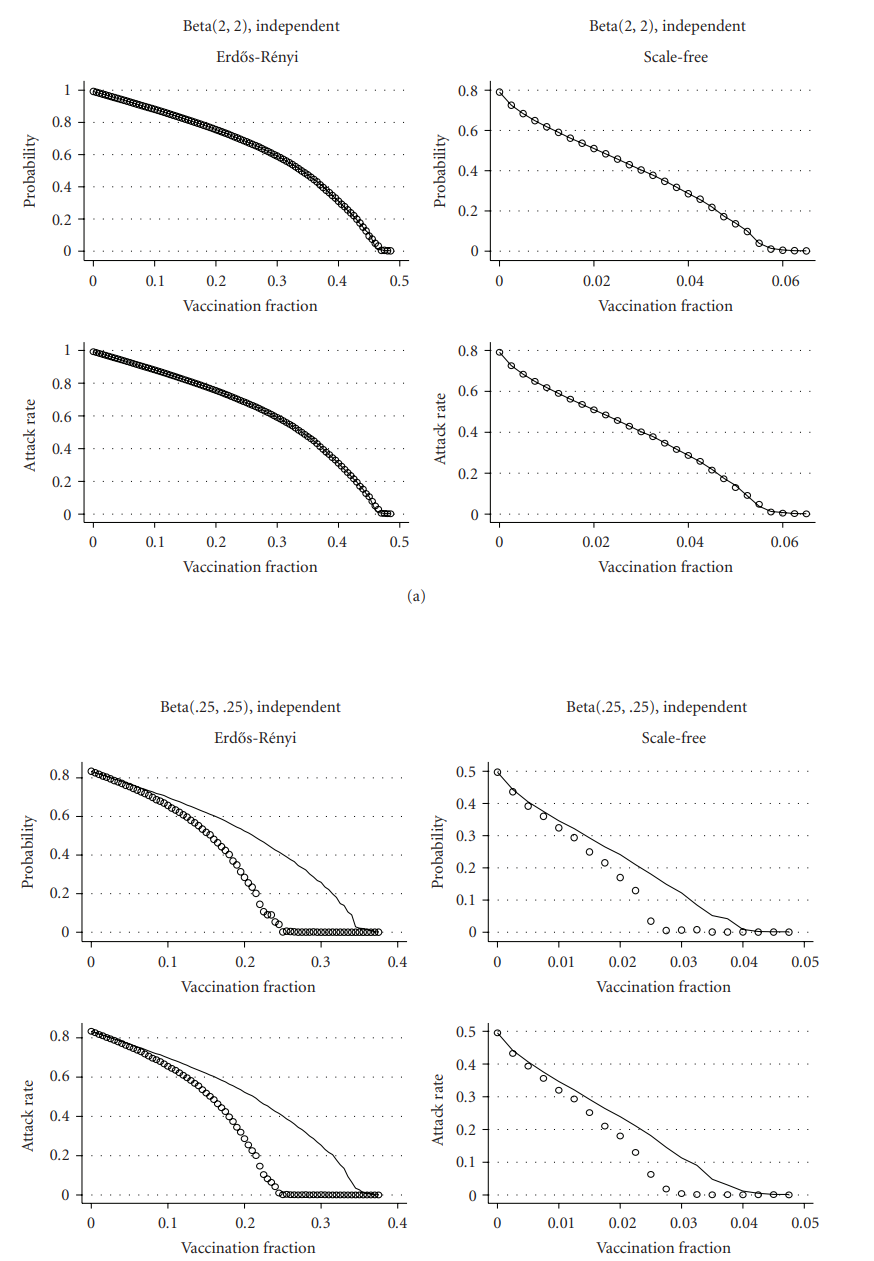
\includegraphics[width=12cm]{3/epigraphs}
  \caption{A comparison of strategy 1 (lines) versus strategy 2 (circles) in reducing the attack rate and probability of an epidemic on Erd\H{o}s-R\'{e}nyi networks and scale-free
    networks. When the infectiousness and susceptibility are beta(2, 2) distributed, both strategies produce nearly identical
  results. When infectiousness and susceptibility are beta(0.25, 0.25) distributed, targeting the GSCC is clearly more effective in reducing both the attack rate and the
probability of an epidemic in both network configurations.\cite{Kenah}}
  \label{fig:epidemiology graphs}
\end{figure}

As is clear from Figure \ref{fig:epidemiology graphs}, strategy 2 of targeting the GSCC is much better at reducing the probability of an epidemic and reducing the attack size of an
epidemic when there's significant variation in the susceptibility and infectiousness of members of the
population. In general, this paper's analysis of vaccination is that vaccinating the highly infectious (i.e. those likely to be in the GIN) will reduce the probability of an
epidemic, and vaccinating the highly susceptible (i.e. those likely to be in the GOUT) will reduce its attack rate. Vaccinating those likely to be in the GSCC will do both. The
major limitation with this model is that it's time-homogeneous meaning that this model cannot account for seasonality, change in behaviour of the population, or the effects of
mitigating strategies that are implemented once a certain level of infection is reached. Say, for example, that vaccination starts after the epidemic has already started, then that
epidemic may not necessarily be modelled accurately by an EPN.
